\documentclass[a4paper]{article}

\usepackage[english]{babel}
\usepackage[utf8]{inputenc}
\usepackage{amsmath}
\usepackage{graphicx}
\usepackage{hyperref}
\usepackage[colorinlistoftodos]{todonotes}
\usepackage{listings}
\usepackage{color}
\usepackage{nameref}
\definecolor{dkgreen}{rgb}{0,0.6,0}
\definecolor{gray}{rgb}{0.5,0.5,0.5}
\definecolor{mauve}{rgb}{0.58,0,0.82}

\lstset{frame=tb,
  language=Python,
  aboveskip=3mm,
  belowskip=3mm,
  showstringspaces=false,
  columns=flexible,
  basicstyle={\small\ttfamily},
  numbers=none,
  numberstyle=\tiny\color{gray},
  keywordstyle=\color{blue},
  commentstyle=\color{dkgreen},
  stringstyle=\color{mauve},
  breaklines=true,
  breakatwhitespace=true,
  tabsize=3
}
\title{Machine Learning Nanodegree  \linebreak Capstone Project}

\author{Marcelo Roger García Escalante}

\date{\today}

\begin{document}
\maketitle

\section{Definition}
%%%%%%%%%%%%%%%%%%%%%%%%%%%%%
\subsection{Project Overview}
%%%%%%%%%%%%%%%%%%%%%%%%%%%%%
% Student provides a high-level overview of the project in layman’s terms. Background information such as the problem domain, the project origin, and related datasets or input data is given.

In layman terms, Machine learning consists of programming the computer to learn from previous data. Today, Machine Learning's method, Deep Reinforcement Learning, is gaining popularity since lots of applications has been given to it, such as Video Games, unmanned vehicles, and control systems. The latter is a well-known field where the goal is to make dynamical systems behave in a desired manner, to achieve this it is required to obtain the mathematical model of the system as explained in \cite{Control}

Since control systems are dynamic, all its environments are modeled as a continuous state space and most of the times as a continuous action space as well. Therefore, it signifies a challenging task to solve by machine learning, some of the algorithms able to tackle these problems are deep Q learning (for infinite state spaces and discrete action spaces), and actor-critic methods (for infinite state and action spaces), both of them being from Deep Reinforcement Learning field. 

In many cases it is not possible to know all the system's features thus it is not possible to get the mathematical model of the system, that is where Deep Reinforcement Learning came in place. There are lots of works developed in Control Systems related to Reinforcement learning. For instance, one approach of Reinforcement Learning applied to Control systems is presented in "A heuristic approach to reinforcement learning control systems" \cite{1098193}

%%%%%%%%%%%%%%%%%%%%%%%%%%%%%%
\subsection{Problem Statement}
%%%%%%%%%%%%%%%%%%%%%%%%%%%%%%
% The problem which needs to be solved is clearly defined. A strategy for solving the problem, including discussion of the expected solution, has been made.

The project aims to solve an OpenAI gym environment from the control section that can be seen here \href{https://gym.openai.com/envs/#classic_control}{Control Environments}. The environment selected is the MountainCar-v0 because it has a continuous state space with a deterministic action space being a good candidate for applying deep q learning. The details of the problem are as follows:
\begin{itemize}
\item \textbf{Task:} MountainCar-v0
\item \textbf{Category:} Classic Control
\item \textbf{Goal:} Get an under powered car to the top of a hill (top = 0.5 position) by creating momentum as shown in Fig.\ref{fig:car}
\begin{figure}[h]
\centering
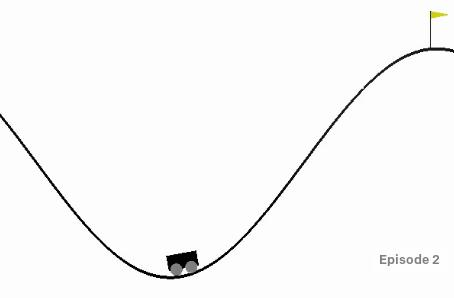
\includegraphics[width=0.8\textwidth]{environment.jpg}
\caption{\label{fig:car} Mountain Car environment}
\end{figure}

\item \textbf{Termination Criteria:} The episode ends when either the goal is reached or 200 actions are made.
\item \textbf{Rewards:} -1 penalty for each environment step until the termination criteria is met.

\item \textbf{Initial state:} The environment starts with the car randomly positioned between -0.6 and -0.4 and always with a velocity of 0.
\item \textbf{Potential Solution:} Since the environment has continuous state space and discrete action space, a good candidate would be a \textbf{Deep Q Network}
\item \textbf{Solution Concerns:} The car will eventually find a solution, however, in order to get an optimal policy in fewer episodes, it might be required to implement Double Deep Q Learning or prioritized memory.

\end{itemize}


%%%%%%%%%%%%%%%%%%%%
\subsection{Metrics}
\label{sub:Metrics}
%%%%%%%%%%%%%%%%%%%%
% Metrics used to measure performance of a model or result are clearly defined. Metrics are justified based on the characteristics of the problem.

\textbf{Average Reward} The main metric for the project will be the average reward in 100 consecutive episodes. The reason to take 100 rewards averaged is to avoid the model to work just for certain specific states in the environment. 
\newline
\textbf{Number of episodes} The secondary metric is the number of episodes in which the problem converges to a solution.

% add here: Why you have chosen to use the 100 episode average performance? Why average them? Why not just choose the 'best'?


% Project Overview
% Problem Statement
% Metrics

\section{Analysis}
\label{sec:analysis}
In this section, an analysis of the data, the algorithms related to the solution and the benchmarks to compare its performance are discussed.
%%%%%%%%%%%%%%%%%%%%%%%%%%%%%
\subsection{Data Exploration}
%%%%%%%%%%%%%%%%%%%%%%%%%%%%%
% If a dataset is present, features and calculated statistics relevant to the problem have been reported and discussed, along with a sampling of the data. In lieu of a dataset, a thorough description of the input space or input data has been made. Abnormalities or characteristics about the data or input that need to be addressed have been identified.
There is no dataset for this project since it involves a Deep Reinforcement Learning approach and learning takes place while running. However, the inputs for the model are the states of the environment which in this case are two continuous measurements: position and velocity of the car as shown in Table\ref{tab:1}, and three actions that are part of the discrete action space shown in Table\ref{tab:action}.

\begin{itemize}
\item \textbf{State Space:}
      \begin{table}[h]
      \centering
      \begin{tabular}{|c|c|c|c|}
      \hline
      \textbf{Num} & \textbf{Observation} & \textbf{Min} & \textbf{Max} \\ \hline
      0            & position             & -1.2         & 0.6          \\ \hline
      1            & velocity             & -0.07        & 0.07         \\ \hline
      \end{tabular}
      \caption{State Space}
      \label{tab:1}
      \end{table}
\item \textbf{Action Space:}
		\begin{table}[h]
        \centering
        \begin{tabular}{|c|c|}
        \hline
        \textbf{Num} & \textbf{Observation} \\ \hline
        0            & push left            \\ \hline
        1            & no push              \\ \hline
        2            & push right           \\ \hline
        \end{tabular}
        \caption{Action Space}
        \label{tab:action}
        \end{table}
\end{itemize}    
%%%%%%%%%%%%%%%%%%%%%%%%%%%%%%%%%%%%%%
\subsection{Exploratory Visualization}
\label{sub:Exploratory}
%%%%%%%%%%%%%%%%%%%%%%%%%%%%%%%%%%%%%%
% A visualization has been provided that summarizes or extracts a relevant characteristic or feature about the dataset or input data with thorough discussion. Visual cues are clearly defined.

As shown in the image below Fig\ref{fig:car_not_normalized} the left edge of the environment is at -1.2 units, the goal of the environment is at 0.5 units represented by the flag, and finally the bottom of the environment is at -0.5 units.

\begin{figure}[h]
\centering
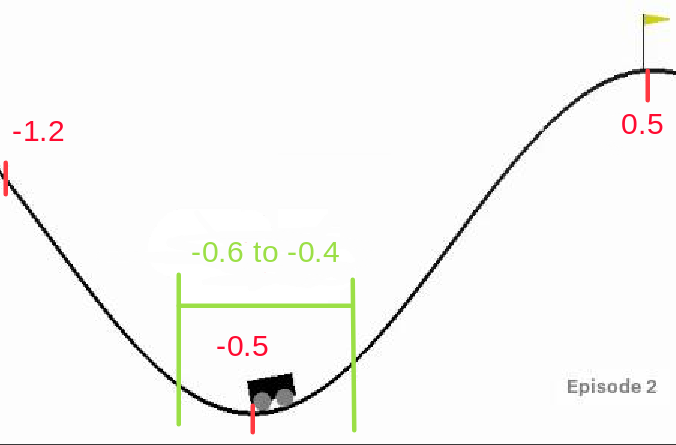
\includegraphics[width=0.8\textwidth]{env_data_visualization.png}
\caption{\label{fig:car_not_normalized} Mountain Car environment key positions}
\end{figure}

On the other hand, as shown in Table\ref{tab:1} velocity's range for the car is from -0.07 and 0.07 thus we can spot out an evident possible issue. Since both the velocity and position are the two variables fed to the deep neural network it is important that both are normalized as explained in this \href{https://www.coursera.org/lecture/deep-neural-network/normalizing-inputs-lXv6U}{video}. Normalizing the data input fed to the deep neural network will enhance optimality of the algorithm since fewer steps for the gradient descent in the loss function will be required as illustrated in Figure\ref{fig:NormVSnotNorm}. Where on the left we can note the function when a data input is not normalized and where is harder for the gradient descent to reach the global minimum, whereas at the right we could observe the function of the same data but this time normalized and in which clearly the gradient descent reaches the minimum smoothly.    

\begin{figure}[h]
\centering
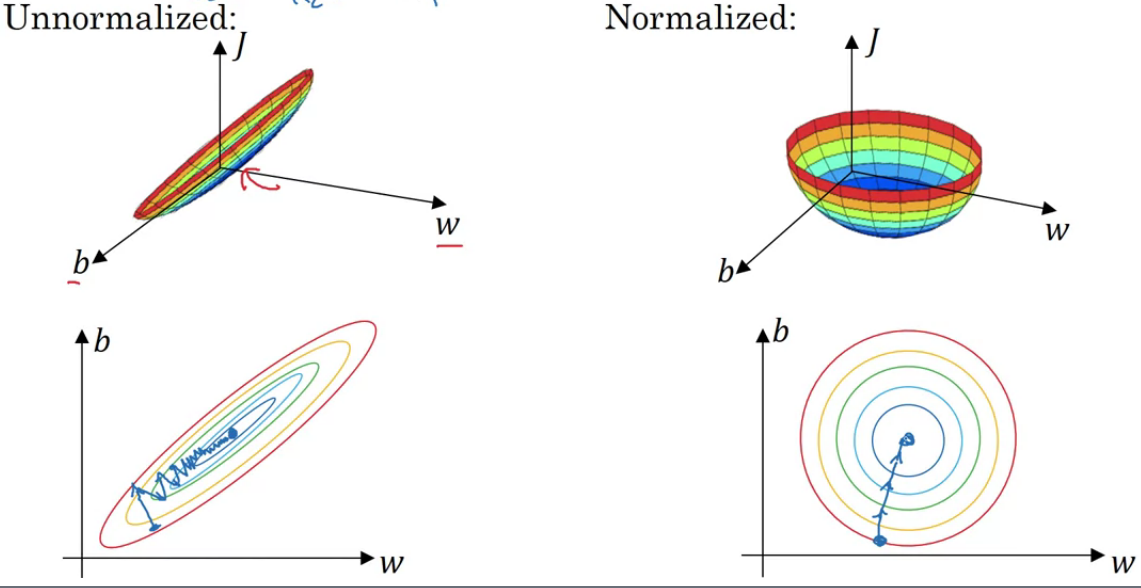
\includegraphics[width=0.8\textwidth]{normalizedVsUnnormalized.png}
\caption{\label{fig:NormVSnotNorm} Unnormalized vs Normalized data \cite{normalizing}}
\end{figure}

%%%%%%%%%%%%%%%%%%%%%%%%%%%%%%%%%%%%%%
\subsection{Deep Q Learning algorithm}
\label{sub:DQN}
%%%%%%%%%%%%%%%%%%%%%%%%%%%%%%%%%%%%%%
% Algorithms and techniques used in the project are thoroughly discussed and properly justified based on the characteristics of the problem. 
As stated in \href{https://storage.googleapis.com/deepmind-media/dqn/DQNNaturePaper.pdf}{DeepMind's paper} the Deep Q Network algorithm should be adequate for any problem where the state space is continuous and the action space discrete. The DQN should follow the following structure:
\begin{itemize}
\item Initialize replay Memory with capacity N
\item Initialize Main Q-network weights $W$ with random uniform distribution.
\item Initialize Target Q-network weights with the main Q-network weights. $W^-\leftarrow W$
\item \textbf{For} the episode in a maximum number of (Episodes):
\begin{itemize}
\item Reset environment
\item Prepare initial state: $S$
\item \textbf{For} time step t in a maximum number of (Steps):
\begin{itemize}
\item[] \underline{\textbf{Observation stage (sample to memory)}}
\item Act in the environment based on state $S$ and get action $A$ using an epsilon-greedy algorithm
\item Take action $A$ and make an environment action-step, get from the output of the environment the new state $S'$ and reward $R$
\item Store the tuple ($S,A,R,S'$) in memory
\item update state. $S \leftarrow S'$
\item[] \underline{\textbf{Learning stage }}\textbf{\dots} 
\item Obtain random mini-batch of tuples from memory. list of ($S,A,R,S'$).
\item Use Target Q-Network to predict the target $Q$ for Main Q-Network for each tuple of the mini-batch. 

$\hat{Q}$=predict($S$)

$\hat{Q}[A]=R+\gamma argMax_a(Q[S',W^-])$
\item Update weights in the Main Q-Network based on the target $\hat{Q}$ as follows: 

$\Delta W=\alpha (Q-\hat{Q}) \nabla_W(\hat{Q})$
\item Update Target Q-network weights with the Main Q-network weights every C steps. $W^-\leftarrow W$
\end{itemize}
\end{itemize}
\end{itemize}

%%%%%%%%%%%%%%%%%%%%%%
\subsection{Benchmark}
\label{sub:Benchmark}
%%%%%%%%%%%%%%%%%%%%%%
% Student clearly defines a benchmark result or threshold for comparing performances of solutions obtained. 

The project has been compared against three benchmarks:
\begin{itemize}
\item \textbf{Random approach}, to ensure the model is better than the most basic model.
\iffalse
\item \textbf{-110 average rewarding}, as stated in \href{https://github.com/openai/gym/wiki/Leaderboard#mountaincar-v0}{OpenAI's documentation} for the MountainCar-v0 the problem pass criteria is a reward of -110 in 100 consecutive episodes
\fi
\item \textbf{Leader board}, as explained in \href{https://github.com/openai/gym/wiki/Leaderboard#mountaincar-v0}{OpenAI's documentation} there are two algorithms that met the -110 average rewarding criteria as shown in Table\ref{tab:crit}. 

\begin{table}[h]
\centering
\begin{tabular}{|c|c|}
\hline
\textbf{User}      & \textbf{Episodes before solve} \\ \hline
jing582            & 1119                           \\ \hline
DaveLeongSingapore & 1967                           \\ \hline
\end{tabular}
\caption{Leader board for the MountainCar-V0 problem}
\label{tab:crit}
\end{table}

\end{itemize}
 % Data Exploration 
 % Exploratory Visualization
 % Algorithms and Techniques
 % Benchmark

\section{Methodology}
%%%%%%%%%%%%%%%%%%%%%%%%%%%%%%%
\subsection{Data Preprocessing}
%%%%%%%%%%%%%%%%%%%%%%%%%%%%%%%
% All preprocessing steps have been clearly documented. Abnormalities or characteristics about the data or input that needed to be addressed have been corrected. If no data preprocessing is necessary, it has been clearly justified.
As spotted out in subsection\nameref{sub:Exploratory}, an issue with the data (our state space) input for the deep neural network is that it is not normalized. This problem could shrink the speed of convergence of our model. Therefore, a pre-process of the data was required, where the input data was converted to a -1 to 1 range instead of the -1.2 to 0.6 for the position, and from -0.07 to 0.07 to -1 to 1 for the velocity. The process is illustrated in the following code snipped: 

\begin{lstlisting}
def normalize_data(self,state):
      position = state[0][0] #getting position from state
      velocity = state[0][1] #getting velocity from state
      state[0][0] = (position + 0.3)/0.9
      state[0][1] = (velocity)/0.07
      return self.state
\end{lstlisting}

As we can note from the code snippet above, the position is added by 0.3 and divided by 0.9 in order to get a -1 to 1 range. On the other hand, the velocity is just divided by its maximum 0.07 value to get a -1 to 1 range as well.

Another featured addressed in the pre-processing stage was the accumulation of previous states into a single one, this idea was borrowed again from \href{https://storage.googleapis.com/deepmind-media/dqn/DQNNaturePaper.pdf}{DeepMind's paper}, where the idea was to stack more states into a single one to obtain additional patterns or relationships between states. The code snippet below shows how this is done.
\begin{lstlisting}

def stateProcessing(self,new_state):
      #This function pre-processes and concatenates last observation with a stack of previous states
      state_history=self.state
      new_state=new_state.reshape(1,2)
      new_state=self.normalize_data(new_state)
      self.state=np.concatenate((state_history[1:],new_state),axis=0)
      return self.state
\end{lstlisting}

%%%%%%%%%%%%%%%%%%%%%%%%%%%
\subsection{Implementation}
%%%%%%%%%%%%%%%%%%%%%%%%%%%
% The process for which metrics, algorithms, and techniques were implemented with the given datasets or input data has been thoroughly documented. Complications that occurred during the coding process are discussed.

The process of implementation of the deep Q learning was built following the steps stated in the \nameref{sub:DQN} section with the following parameters introduced:
\begin{itemize}
\item \textbf{Number of episodes:} 4000
\item \textbf{Maximum number of steps per episode:} 200 (limited by the environment)
\item \textbf{Number of stacked states:} None
\item \textbf{Number of episodes to update target model's weights:} 6
\item \textbf{Replay memory structure type:} Deque
\item \textbf{Memory size:} 5000
\item \textbf{Mini-batch size for training:} 128
\item \textbf{$\gamma$:} 0.99
\item \textbf{Initial $\epsilon$:} 1.0
\item \textbf{$\epsilon$ decay factor:} 0.99
\item \textbf{Minimum $\epsilon$ value:} 0.01
\item \textbf{Learning rate:} 0.005
\item \textbf{Deep Q Network implemented:}
    \begin{itemize}
    \item \textbf{input shape} = (number of stacked states)+state space size
    \item A fully connected \textbf{hidden layer} (Dense layer) with \textbf{200 nodes}.
    \item \textbf{Uniform} initialization of weights 
    \item \textbf{L2 regularizer} with a 0.01 weight
    \item \textbf{Batch normalization} layer
    \item \textbf{Relu} activation layer
    \item \textbf{Output layer} with shape = action space size with a \textbf{linear} activation
    \item \textbf{Loss function:} mean square error
    \item \textbf{Optimizer: } Adam
    \end{itemize}
\end{itemize}


%%%%%%%%%%%%%%%%%%%%%%%
\subsection{Refinement}
\label{sub:Refinement}
%%%%%%%%%%%%%%%%%%%%%%%
% The process of improving upon the algorithms and techniques used is clearly documented. Both the initial and final solutions are reported, along with intermediate solutions, if necessary.

After implementation of the Q learning algorithm the main problem faced was the long training required for first convergence in a solution. The problem was due to the configuration of the environment since the most visited states were at the bottom because of gravity pulling the car down. Therefore, a lot of the episodes were occupied just on the exploration stage, otherwise, the algorithm would not find a solution and if it founds it, it diverged again after a couple of episodes later. 

\vspace{0.5cm}

\textbf{1.} An alternative solution implemented to catalyze the convergence of the algorithm was to use a custom reward function, as shown in the following pseudo code:

\begin{itemize}
\item[] \textbf{IF} current position of the car = Goal position
\item[] \quad \textbf{Reward} event
\item[] \textbf{IF} current position of the car = Left edge of the environment
\item[] \quad \textbf{Punish} event
\item[] \textbf{IF} car ascending and velocity produced is contrary to the action. (E.g. action applied is right but the car goes left due to gravity)
\item[] \quad \textbf{Punish} event
\item[] \textbf{IF} car's speed is high and suddenly drops due to an action
\item[] \quad \textbf{Punish} event
\end{itemize}

The result of this custom reward system was a significant increase in the speed of convergence of the algorithm from more than 1000 to 400 episodes.
\linebreak

\textbf{2.} Another important achievement in velocity of convergence was the implementation of a skipping frames system, which was inspired from the \href{https://storage.googleapis.com/deepmind-media/dqn/DQNNaturePaper.pdf}{DeepMind's paper}, where they skipped frames to speed up the training process of the Atari images fed to its neural network. The skipped frames were set to 4, this means that the same action was applied to the next four states. The result was a huge 
increase in the speed of convergence, that in conjunction with the custom reward system dropped the 400 episodes to 200 episodes.
% Data Preprocessing
% Implementation
% Refinement

\section{Results}
In this section, the results of the model applied to the environment are illustrated. The first sub-section shows an evaluation of the model based on the metrics stated in \nameref{sub:Metrics}. The last sub-section shows a Justification of the model, which is a comparison of its performance against the \nameref{sub:Benchmark}.
%%%%%%%%%%%%%%%%%%%%%%%%%%%%%%%%%%%%%%%%%%%%
\subsection{Model Evaluation and Validation}
%%%%%%%%%%%%%%%%%%%%%%%%%%%%%%%%%%%%%%%%%%%%
% The final model’s qualities — such as parameters — are evaluated in detail. Some type of analysis is used to validate the robustness of the model’s solution.
The reason to implement a custom reward (CR) + skipped frames (SF) system as explained in \nameref{sub:Refinement}  was to favor the creation of momentum. Momentum is the key physical attribute to solve this environment which at the same time is proportional to the speed of the car and its mass. However, since we do not have control over its mass, the only variable to favor in the environment is velocity, that is why all CR + SF focus on increasing the speed of the car. The results compared to a normal environment reward (ER) after the implementation of the DQN are shown in Table\ref{tab:CR+SF}.
\begin{table}[h]
\centering
\begin{tabular}{|c|c|c|c|}
\hline
                                                                                             & \textbf{\begin{tabular}[c]{@{}c@{}}Environment's\\ Reward (ER)\end{tabular}} & \textbf{\begin{tabular}[c]{@{}c@{}}ER+Custom\\ Reward (CR)\end{tabular}} & \textbf{\begin{tabular}[c]{@{}c@{}}CR+Skipped\\ Frames (SF)\end{tabular}} \\ \hline
\textbf{\begin{tabular}[c]{@{}c@{}}Episodes required to\\ find a solution\end{tabular}}      & \textgreater 2000                                                            & \textgreater 400                                                         & \textgreater 200                                                     \\ \hline
\textbf{\begin{tabular}[c]{@{}c@{}}Best 100 average \\ Reward in 2000 episodes\end{tabular}} & $<$ -190                                                                          & -160 to -150                                                               & -130 to -120                                                           \\ \hline
\end{tabular}
\caption{ER vs CR+SF}
\label{tab:CR+SF}
\end{table}

.

%%%%%%%%%%%%%%%%%%%%%%%%%%
\subsection{Justification}
%%%%%%%%%%%%%%%%%%%%%%%%%%
% The final results are compared to the benchmark result or threshold with some type of statistical analysis. Justification is made as to whether the final model and solution is significant enough to have adequately solved the problem.

The results of the model against the benchmarks stated for this projects are presented in Table\ref{tab:modelVSbenchmarks}

\begin{table}[h]
\centering
\begin{tabular}{|c|c|c|c|c|}
\hline
                                                                                                   & \textbf{\begin{tabular}[c]{@{}c@{}}Random\\ algorithm\end{tabular}} & \textbf{\begin{tabular}[c]{@{}c@{}}First in Leader\\ Board (jing582)\end{tabular}} & \textbf{\begin{tabular}[c]{@{}c@{}}Second in Leader\\ Board \\ (DaveLeong)\end{tabular}} & \textbf{DQN Model} \\ \hline
\textbf{\begin{tabular}[c]{@{}c@{}}Episodes required \\ to converge \\ to a solution\end{tabular}} & \begin{tabular}[c]{@{}c@{}}No solution\\ Found\end{tabular}         & 1119                                                                               & 1967                                                                                     & $<$1000               \\ \hline
\textbf{\begin{tabular}[c]{@{}c@{}}100 average \\ range in Testing \\ the algorithm\end{tabular}}  & -200                                                                & \textgreater  -110                                                                  & \textgreater  -110                                                                        & -130 to -120       \\ \hline
\end{tabular}
\caption{Deep Q learning model against Benchmarks}
\label{tab:modelVSbenchmarks}
\end{table}
As it can be seen in the table above, our model is much better than a random algorithm where the 100 average in testing is -200, whereas the DQN model result is between -130 and -120. On the other hand, both leaders got better 100 average results than the DQN model. However, the speed of convergence of the DQN was faster, since it required less than 1000 episodes to converge to a solution. Overall we can state that the DQN is a good candidate to solve the Mountain Car problem, and to strengthen the statement we could find the graph of the learning process of the model in Figure\ref{fig:Learning}

\begin{figure}[h]
\centering
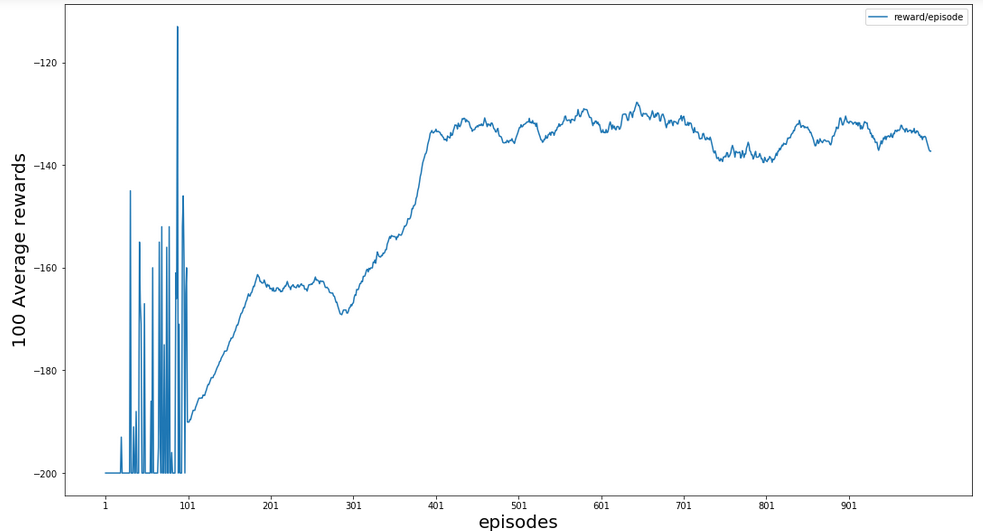
\includegraphics[width=0.8\textwidth]{LearningProcessDQN.png}
\caption{Learning process of the Deep Q learning approach to the Mountain Car problem}
\label{fig:Learning} 
\end{figure}

.

% Model Evaluation and Validation
% Justification

\section{Conclusion}
% A visualization has been provided that emphasizes an important quality about the project with a thorough discussion. Visual cues are clearly defined.
% Student adequately summarizes the end-to-end problem solution and discusses one or two particular aspects of the project they found interesting or difficult.
This project has turned out to be more challenging than expected. The first problem to overcome was the lack of a GPU to work with the neural network which delayed the training process. Therefore, the work done in this project focused more on enhancing the speed of convergence of the algorithm rather than getting a better 100 reward average. The other main conflict faced in this project was the lack of states visited at the beginning of the training process, since the car tended to visit more the bottom of the mountain due to gravity pulling down the car, that was what delayed the training process the most. At the end, generating an additional custom reward of the environment plus skipping frames turned to be the key features to overcome these problems, where the approach was to build a Deep Q Learning model the more simplistic possible to solve the problem since a more complex model should lead to a better 100 average reward value but at the cost of more computational resources. Overall the project highlighted the importance of an optimal algorithm, where the goal was to learn more from less information of the environment (i.e. fewer episodes required). Finally, to visualize the outcome of the last 100 average reward training of the model a video was generated which can be seen \href{https://youtu.be/PxzqPLuuu5o}{Here}.
%%%%%%%%%%%%%%%%%%%%%%%%%%%%%%%%
\subsection{Future Improvements}
%%%%%%%%%%%%%%%%%%%%%%%%%%%%%%%%

% Discussion is made as to how one aspect of the implementation could be improved. Potential solutions resulting from these improvements are considered and compared/contrasted to the current solution.

There is plenty of space to enhance the performance of this project. Some of the possible ideas are the following:
\begin{itemize}
\item Try training the model with a more complex deep neural network, perhaps one more hidden layer.
\item Try a DDQN, the model created for this project already has implemented an option for a Double Deep Q Learning process. It will demand more computational resources but it must perform better, especially at the beginning of the training process.
\item Try to implement prioritized memory since one of the main problems stated in the training process was the lack of new states to learn from, a prioritized memory should help overcome this issue since it will tend to select the new states or the states from which it will learn more.
\item Try stacked states, the model created has already implemented the option to stack more states into the Deep Neural Network. This idea was brought from DeepMind's paper where four Atari frames were stacked into a single state to learn additional patterns and features from the environment. \cite{mnih2015humanlevel}
\end{itemize}
% Free-Form Visualization
% Reflection
% Improvement


\vspace*{1cm}
\bibliographystyle{apalike}
\bibliography{bibliography}
\end{document}